\documentclass[answers]{exam}
\makeindex

\usepackage{amsmath, amsfonts, amssymb, amstext, amscd, amsthm, makeidx, graphicx, hyperref, url, enumerate}
\newtheorem{theorem}{Theorem}
\allowdisplaybreaks

\begin{document}

\begin{center}
{\Large CS 156a - Problem Set 4} \\
\medskip
Marco Yang \\
\medskip
2237027
\bigskip
\end{center}

\section*{Generalization Error}

\begin{questions}
\question
For an $\mathcal{H}$ with $d_{vc} = 10$, if you want 95\% confidence that your generalization 
error is at most 0.05, what is the closest numerical approximation of the sample 
size that the VC generalization bound predicts?
\begin{choices}
    \choice 400,000
    \choice 420,000
    \choice 440,000
    \choice 460,000
    \choice 480,000
\end{choices}

\begin{solution}
D. 460,000

Upon graphing the probability error bound, we get that it occurs at around
480,000.
\end{solution}

\question
There are a number of bounds on the generalization error $\epsilon$, all holding 
with probability at least $1 - \delta$. Fix $d_{vc} = 50$ and $\delta = 0.05$ and 
plot these bounds as a function of $N$. Which bound is the smallest for very large 
$N$, say $N = 10,000$? Note that [c] and [d] are implicit bounds in $\epsilon$.
\begin{choices}
    \choice Original VC bound: 
    $\epsilon \leq \sqrt{\frac{8}{N} \ln \frac{4m_H(2N)}{\delta}}$
    \choice Rademacher Penalty Bound: 
    $\epsilon \leq \sqrt{\frac{2 \ln(2Nm_H(N))}{N}} + 
    \sqrt{\frac{2}{N} \ln \frac{1}{\delta}} + \frac{1}{N}$
    \choice Parrondo and Van den Broek: 
    $\epsilon \leq \sqrt{\frac{1}{N} \left(2\epsilon + \ln 
    \frac{6m_H(2N)}{\delta}\right)}$
    \choice Devroye: 
    $\epsilon \leq \sqrt{\frac{1}{2N} \left(4\epsilon(1 + \epsilon) + 
    \ln \frac{4m_H(N^2)}{\delta}\right)}$
    \choice They are all equal.
\end{choices}

\begin{solution}
D. Devroye 

% 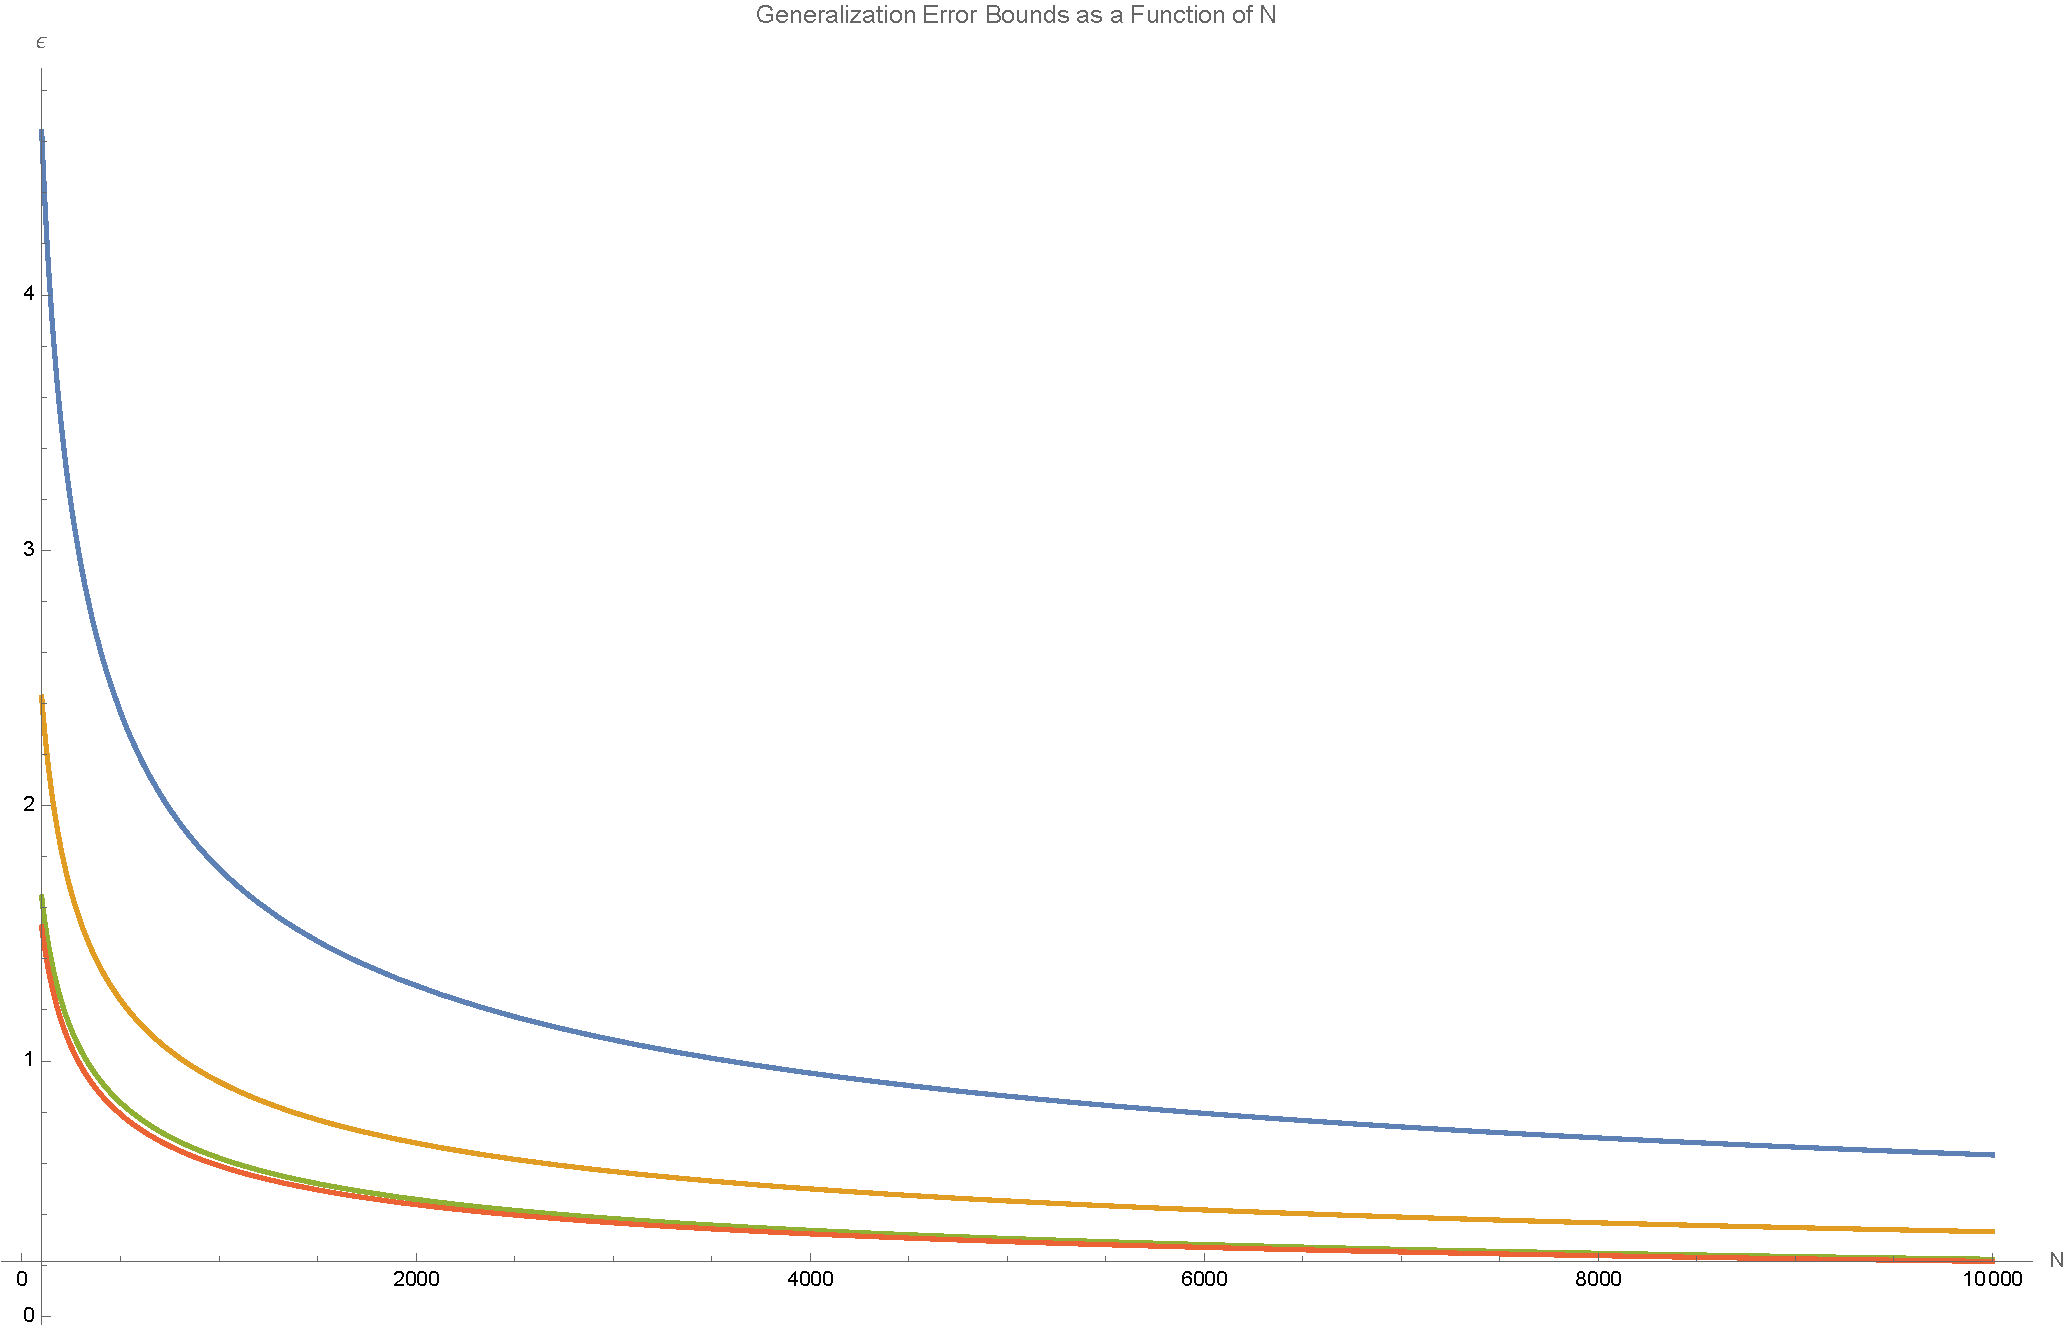
\includegraphics[width=\textwidth]{img/p4-2.pdf}
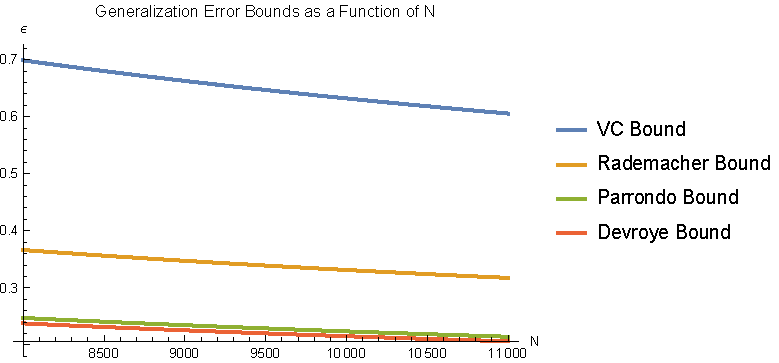
\includegraphics[width=\textwidth]{img/p4-2-zoom.pdf}
\end{solution}

\question
For the same values of $d_{vc}$ and $\delta$ of Problem 2, but for small $N$, say 
$N = 5$, which bound is the smallest?
\begin{choices}
    \choice Original VC bound: 
        $\epsilon \leq \sqrt{\frac{8}{N} \ln \frac{4m_H(2N)}{\delta}}$
    \choice Rademacher Penalty Bound: 
        $\epsilon \leq \sqrt{\frac{2 \ln(2Nm_H(N))}{N}} + 
        \sqrt{\frac{2}{N} \ln \frac{1}{\delta}} + \frac{1}{N}$
    \choice Parrondo and Van den Broek: 
        $\epsilon \leq \sqrt{\frac{1}{N} \left(2\epsilon + \ln 
        \frac{6m_H(2N)}{\delta}\right)}$
    \choice Devroye: 
        $\epsilon \leq \sqrt{\frac{1}{2N} \left(4\epsilon(1 + \epsilon) + 
        \ln \frac{4m_H(N^2)}{\delta}\right)}$
    \choice They are all equal.
\end{choices}

\begin{solution}
C. Parrondo

% 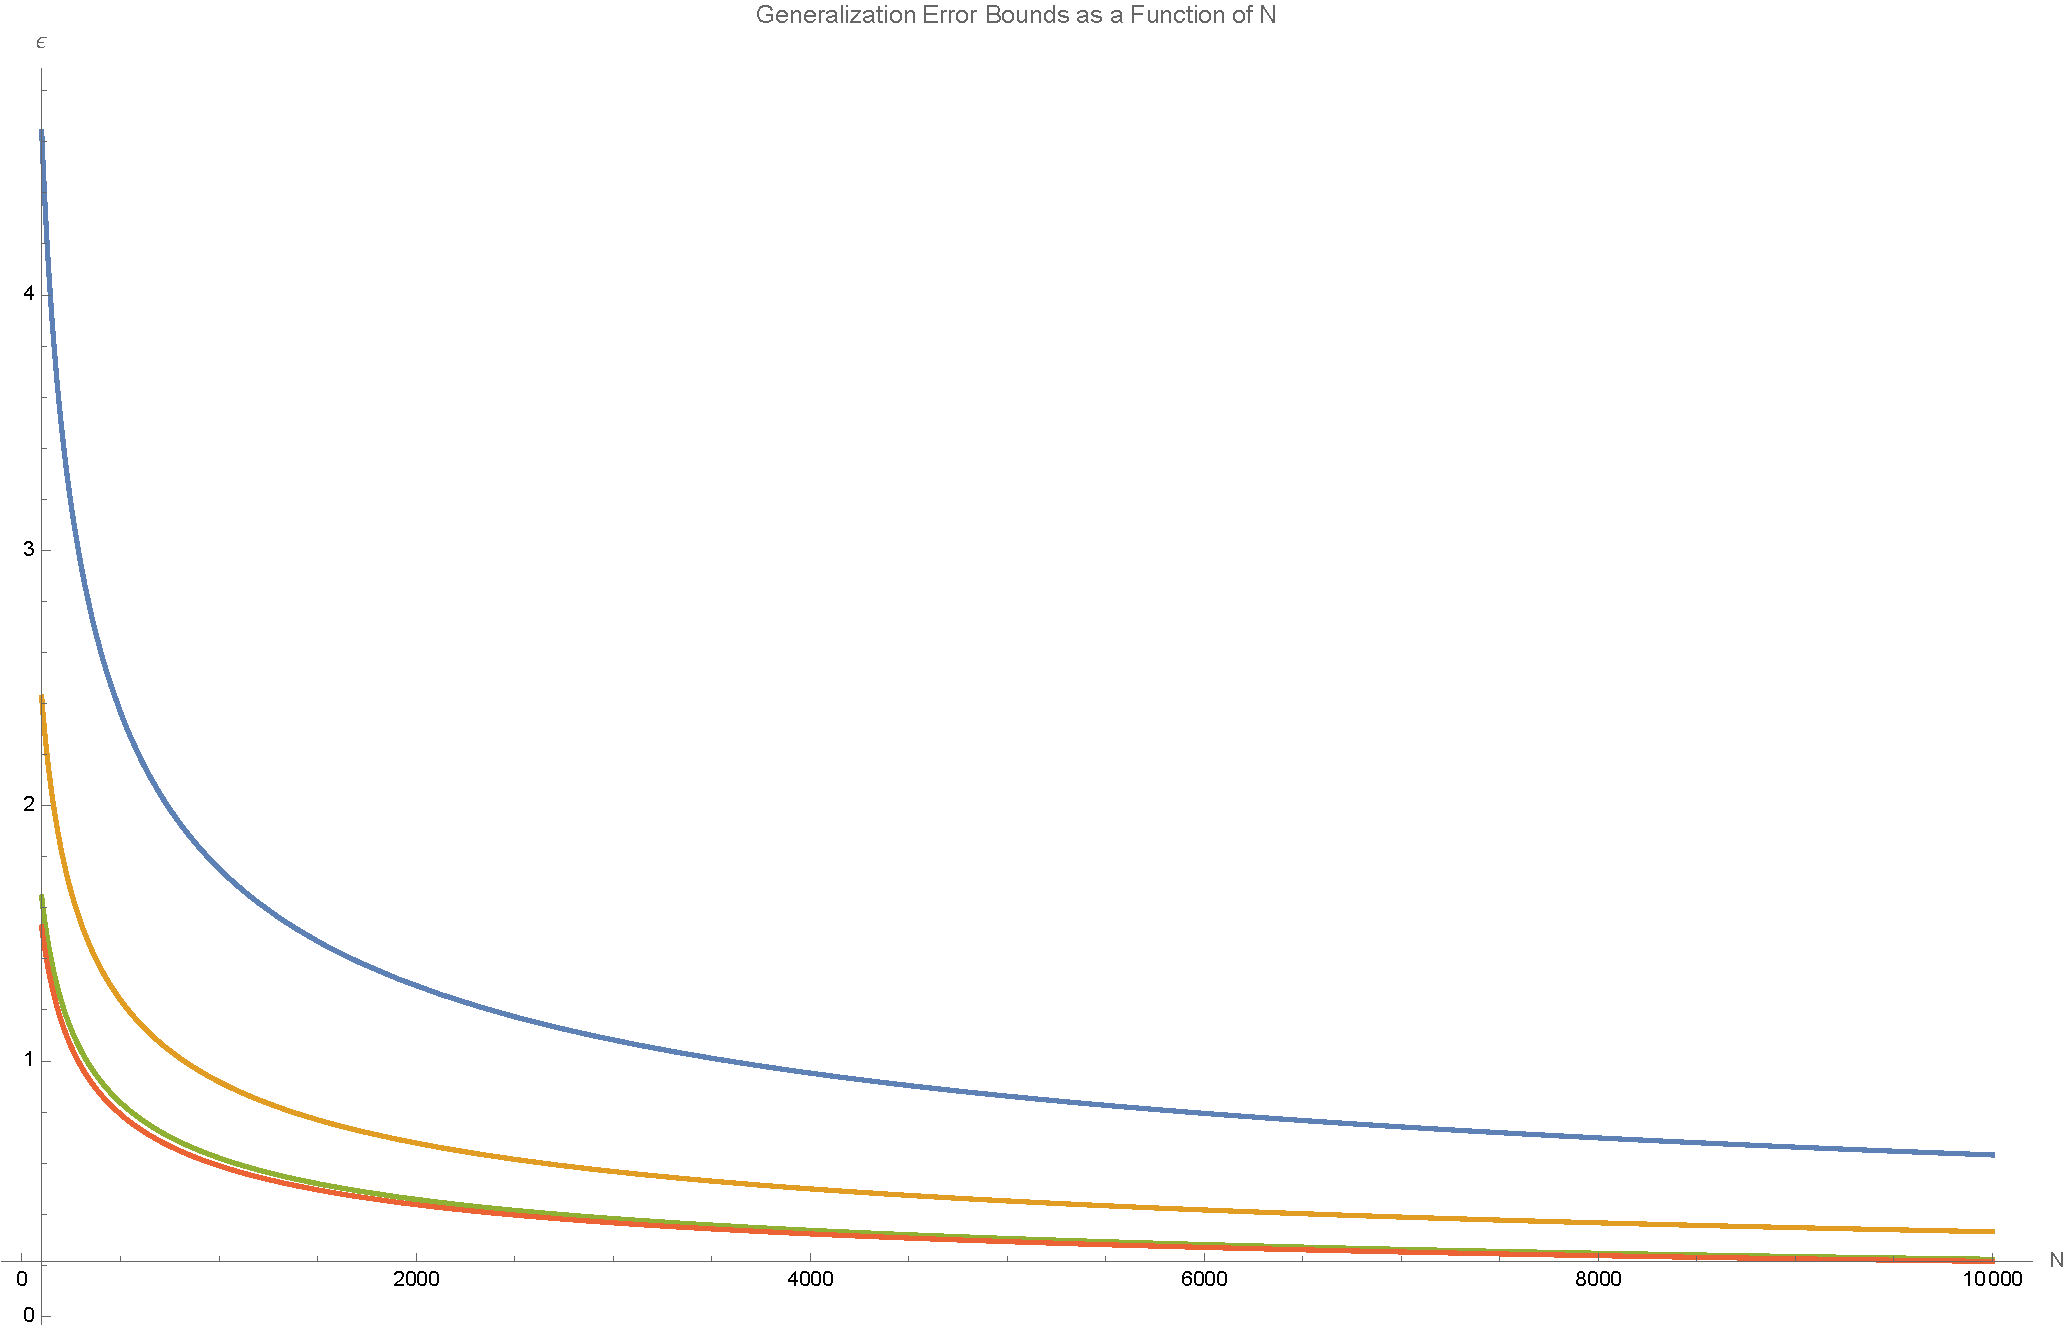
\includegraphics[width=\textwidth]{img/p4-2.pdf}
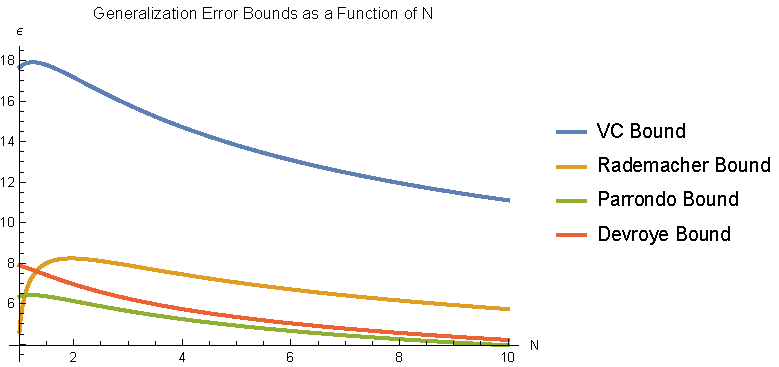
\includegraphics[width=\textwidth]{img/p4-3-zoom.pdf}
\end{solution}
\end{questions}

\section*{Bias and Variance}

Consider the case where the target function $f:[-1, 1] \to \mathbb{R}$ is
given by $f(x) = \sin(\pi x)$ and the input probability distribution is
uniform on $[-1, 1]$. Assume that the training set has only two examples
(picked independently), and that the learning algorithm produces the
hypothesis that minimizes the mean squared error on the examples.

\begin{questions}
\setcounter{question}{3}
\question
Assume the learning model consists of all hypotheses of the form $h(x) = ax$. 
What is the expected value, $\bar{g}(x)$, of the hypothesis produced by the 
learning algorithm (expected value with respect to the data set)? Express your 
$\bar{g}(x)$ as $\hat{a}x$, and round $\hat{a}$ to two decimal digits only, then 
match exactly to one of the following answers.
\begin{choices}
    \choice $\bar{g}(x) = 0$
    \choice $\bar{g}(x) = 0.79x$
    \choice $\bar{g}(x) = 1.07x$
    \choice $\bar{g}(x) = 1.58x$
    \choice None of the above
\end{choices}

\begin{solution}
Given $x_1, x_2 \in [-1, 1]$, the formula for MSE is 

\[
E = \frac{1}{2}\left( (\sin(\pi x_1) - ax_1)^2 + (\sin(\pi x_2) - ax_2)^2 \right)
.\] 

The optimal value of the slope $a$ occurs when the 

\[
\frac{\partial E}{\partial a} = 0 \implies a = \frac{x_1\sin(\pi x_1) + x_2\sin(\pi x_2)}{x_1^2 + x_2^2}
.\] 

The expected value of $a$ is

\[
\frac{1}{(1 - (-1)) + (1 - (-1))} \int_{-1}^{1} \int_{-1}^{1} a(x_1,x_2) \, dx_1 \, dx_2 \approx 1.42
.\] 

Thus, our answer is E. None of the above.
\end{solution}

\question
What is the closest value to the bias in this case?
\begin{choices}
    \choice 0.1
    \choice 0.3
    \choice 0.5
    \choice 0.7
    \choice 1.0
\end{choices}

\begin{solution}
\begin{align*}
    \text{bias} &= \mathbb{E}\left[ (\overline{g}(x) - f(x))^2 \right] \\ 
    &= \int_{-1}^{1} \frac{1}{2}(ax_1 - \sin(\pi x_1))^2 \, \frac{dx_1}{1 - (-1)} + 
    \int_{-1}^{1} \frac{1}{2}(ax_2 - \sin(\pi x_2))^2 \, \frac{dx_2}{1 - (-1)} \\
    &\approx 0.27
.\end{align*}

B. 0.3
\end{solution}

\question
What is the closest value to the variance in this case?
\begin{choices}
    \choice 0.2
    \choice 0.4
    \choice 0.6
    \choice 0.8
    \choice 1.0
\end{choices}

\begin{solution}
Using our formula from earlier for the slope given two randomly chosen points
and the average hypothesis we found earlier, the expected value of 
the error between a random hypothesis and the average hypothesis
is the integral over the 2 random points for the slope and the two random 
points for the input. Since the two random input inputs are iid,

\begin{align*}
    \text{var} &= 2 \cdot \int_{-1}^{1} \int_{-1}^{1} \int_{-1}^{1} \frac{1}{2}(a(x_1,x_2)x_3 - ax_3)^2 \, \frac{dx_1}{2} \, \frac{dx_2}{2} \, \frac{dx_3}{2} \\ 
    &\approx 0.23
.\end{align*}

B. 0.2
\end{solution}

\question
Now, let’s change $\mathcal{H}$. Which of the following learning models has the 
least expected value of out-of-sample error?
\begin{choices}
    \choice Hypotheses of the form $h(x) = b$
    \choice Hypotheses of the form $h(x) = ax$
    \choice Hypotheses of the form $h(x) = ax + b$
    \choice Hypotheses of the form $h(x) = ax^2$
    \choice Hypotheses of the form $h(x) = ax^2 + b$
\end{choices}

\begin{solution}
A. Hypotheses of the form $h(x) = b$

The less complex a hypothesis, the better it generalizes.
\end{solution}
\end{questions}

\section*{VC Dimension}

\begin{questions}
\setcounter{question}{7}
\question
Let $q \geq 1$ be an integer, and assume that $m_{\mathcal{H}}(1) = 2$. What is 
the VC dimension of a hypothesis set whose growth function for all $N \geq 1$ 
satisfies: $m_{\mathcal{H}}(N + 1) = 2m_{\mathcal{H}}(N) - \binom{N}{q}$? Recall 
that $\binom{M}{m} = 0$ when $m > M$.
\begin{choices}
    \choice $q - 2$
    \choice $q - 1$
    \choice $q$
    \choice $q + 1$
    \choice None of the above
\end{choices}

\begin{solution}
Writing out the growth function in terms of $d_{\text{VC}}$, we have

\[
\sum_{i=0}^{d_{\text{VC}}} \binom{N+1}{i} = 2 \sum_{i=0}^{d_{\text{VC}}} \binom{N}{i} - \binom{N}{q}
.\] 

Notice that the pattern in Pascal's Triangle dictates that

\[
\binom{N+1}{i} = \binom{N}{i-1} = \binom{N}{i}
.\] 

Thus,

\[
\sum_{i=0}^{d_{\text{VC}}} \binom{N+1}{i} = 2 \sum_{i=0}^{d_{\text{VC}}} \binom{N}{i} - \binom{N}{d_{\text{VC}}}
.\] 

Thus, our answer is C. $d_{\text{VC}} = q$.
\end{solution}

\question
For hypothesis sets $\mathcal{H}_{1}, \mathcal{H}_2, \ldots, \mathcal{H}_K$ 
with finite, positive VC dimensions $d_{vc}(\mathcal{H}_k)$ (same input 
space $X$), some of the following bounds are correct and some are not. Which, 
among the correct ones, is the tightest bound (the smallest range of values) 
on the VC dimension of the intersection of the sets: $d_{vc}(\cap_{k=1}^K 
\mathcal{H}_k)$? (The VC dimension of an empty set or a singleton set is 
taken as zero.)
\begin{choices}
    \choice $0 \leq d_{\text{VC}}(\cap_{k=1}^K \mathcal{H}_k) \leq \sum_{k=1}^K d_{\text{VC}}(\mathcal{H}_k)$
    \choice $0 \leq d_{\text{VC}}(\cap_{k=1}^K \mathcal{H}_k) \leq \min\{d_{\text{VC}}(\mathcal{H}_k)\}_{k=1}^K$
    \choice $0 \leq d_{\text{VC}}(\cap_{k=1}^K \mathcal{H}_k) \leq \max\{d_{\text{VC}}(\mathcal{H}_k)\}_{k=1}^K$
    \choice $\min\{d_{\text{VC}}(\mathcal{H}_k)\}_{k=1}^K \leq d_{\text{VC}}(\cap_{k=1}^K \mathcal{H}_k) \leq 
    \max\{d_{\text{VC}}(\mathcal{H}_k)\}_{k=1}^K$
    \choice $\min\{d_{\text{VC}}(\mathcal{H}_k)\}_{k=1}^K \leq d_{\text{VC}}(\cap_{k=1}^K \mathcal{H}_k) \leq 
    \sum_{k=1}^K d_{\text{VC}}(\mathcal{H}_k)$
\end{choices}

\begin{solution}
B. 

In the case that the intersection is an empty set, $d_{\text{VC}}=0$. The best
case scenario is that the intersection contains all the hypotheses in the 
least robust set; we can prove this by contradiction. Assume that the 
intersection contained all the hypothesis in a non-least-robust set 
$\mathcal{H}_{i}$. Then, that means there is another set that is a least robust
set $\mathcal{H}_{j}$ robust with all the hypotheses in the $\mathcal{H}_{i}$.
However, this contradicts the definition of $\mathcal{H}_{j}$ as being
the least robust since it is at least as robust as $\mathcal{H}_{i}$. Thus,
the intersection can at best be as robust as the least robust subset.
\end{solution}

\question
For hypothesis sets $H_1, H_2, \ldots, H_K$ with finite, positive VC dimensions 
$d_{vc}(H_k)$ (same input space $X$), some of the following bounds are correct 
and some are not. Which, among the correct ones, is the tightest bound (the 
smallest range of values) on the VC dimension of the union of the sets: 
$d_{vc}(\cup_{k=1}^K H_k)$?

\begin{choices}
    \choice $0 \leq d_{vc}(\cup_{k=1}^K H_k) \leq \sum_{k=1}^K d_{vc}(H_k)$
    \choice $0 \leq d_{vc}(\cup_{k=1}^K H_k) \leq K - 1 + \sum_{k=1}^K 
    d_{vc}(H_k)$
    \choice $\min\{d_{vc}(H_k)\}_{k=1}^K \leq d_{vc}(\cup_{k=1}^K H_k) \leq 
    \sum_{k=1}^K d_{vc}(H_k)$
    \choice $\max\{d_{vc}(H_k)\}_{k=1}^K \leq d_{vc}(\cup_{k=1}^K H_k) \leq 
    \sum_{k=1}^K d_{vc}(H_k)$
    \choice $\max\{d_{vc}(H_k)\}_{k=1}^K \leq d_{vc}(\cup_{k=1}^K H_k) \leq 
    K - 1 + \sum_{k=1}^K d_{vc}(H_k)$
\end{choices}

\begin{solution}
D. $\max\{d_{vc}(H_k)\}_{k=1}^K \leq d_{vc}(\cup_{k=1}^K H_k) \leq 
    \sum_{k=1}^K d_{vc}(H_k)$

The size of the union $A \cup B$ of 2 hypotheses sets $A$ and $B$ is
$|A| + |B|$. By definition of VC dimension,

\begin{gather*}
2^{d_{VC}(A)} \le |A| < 2^{d_{VC}(A) + 1} \\ 
2^{d_{VC}(B)} \le |B| < 2^{d_{VC}(B) + 1}
\end{gather*}

Since $2^{a} + 2^{b} \le 2^{a + b}$ for positive $a, b$,

\[
\text{max}(2^{d_{VC}(A)}, 2^{d_{\text{VC}}(B)}) \le |A| + |B| \le 2^{d_{\text{VC}}(A) + d_{\text{VC}}(B)}
.\] 
\end{solution}

\end{questions}

\end{document}
